\chapter{MVP Boundaries, UML Schematics, and Architectural Topologies}
\label{chap:architecture}

This chapter presents the architectural design of the Lectura platform through UML diagrams and system schematics. It begins by defining the scope of the minimum viable product, then documents the system architecture, key interaction flows, and the database structure.

\section{Minimum Viable Product (MVP) Scope}
The MVP scope for Lectura was kept deliberately narrow to validate the core idea without unnecessary complexity. The features included in the initial release were: user registration and authentication, multimedia file upload, real-time transcript extraction, automated generation of study artifacts (summaries, quizzes, flashcards, and presentations), and a persistent content library on the frontend. More advanced features such as detailed analytics dashboards and offline synchronization were deferred to future development phases.

\section{System Architecture Overview}
The overall system architecture is documented in Figure~\ref{fig:sys_architecture}. Lectura follows a three-tier architecture: a Client Presentation Layer built with React, an Application Logic Layer implemented in Go, and a Data/Generation Layer consisting of PostgreSQL, Redis, and the Google Gemini API.

\begin{figure}[htbp]
\centering
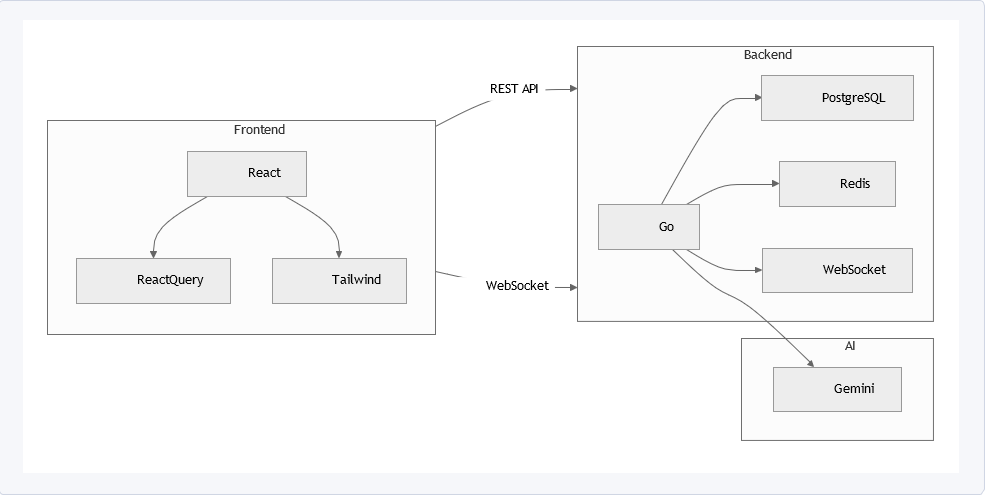
\includegraphics[width=\textwidth]{chapters/chapter05/images/sys_architecture.png}
\caption{System Architecture Diagram showing the three-tier application structure.}
\label{fig:sys_architecture}
\end{figure}

\section{Use Case Diagram}
Figure~\ref{fig:use_case} shows the main interaction paths within the application. The diagram distinguishes between actions available to unauthenticated visitors (such as viewing the landing page) and those available to logged-in users (such as uploading content and generating study materials).

\begin{figure}[htbp]
\centering
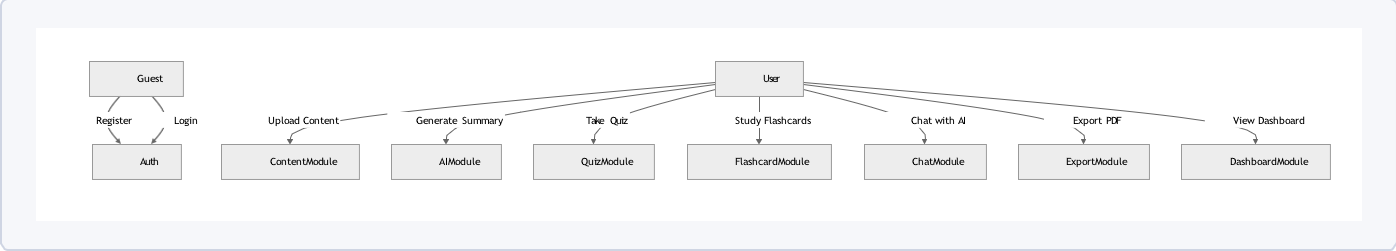
\includegraphics[width=0.9\textwidth]{chapters/chapter05/images/image2.png}
\caption{Use Case Diagram showing interactions between users and system features.}
\label{fig:use_case}
\end{figure}

\section{Content Generation Sequence Diagram}
Because calls to external LLM APIs can take 10--60 seconds, the generation process is handled asynchronously. Figure~\ref{fig:sequence_gen} traces the full sequence: the user submits content from the React frontend, the Go backend creates a job and places it in the Redis queue, a background worker picks up the job and sends requests to the Gemini API, and finally the results are stored in PostgreSQL and the user is notified via a WebSocket message.

\begin{figure}[htbp]
\centering
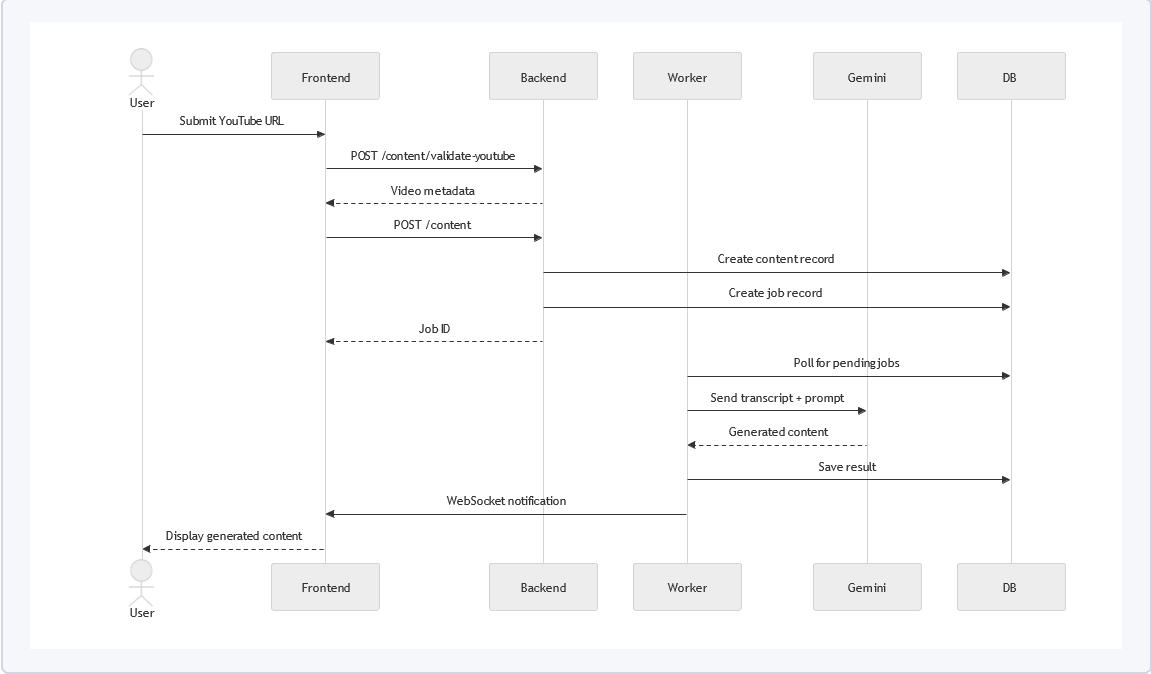
\includegraphics[width=\textwidth]{chapters/chapter05/images/image3.png}
\caption{Sequence Diagram for asynchronous content generation via the LLM API.}
\label{fig:sequence_gen}
\end{figure}

\section{Authentication Sequence Diagram}
Figure~\ref{fig:auth_matrix} illustrates the authentication flow. It covers the OAuth login process, JWT token signing on the backend, the issuance of secure HttpOnly refresh tokens, and the subsequent token validation that occurs on each authenticated API request.

\begin{figure}[htbp]
\centering
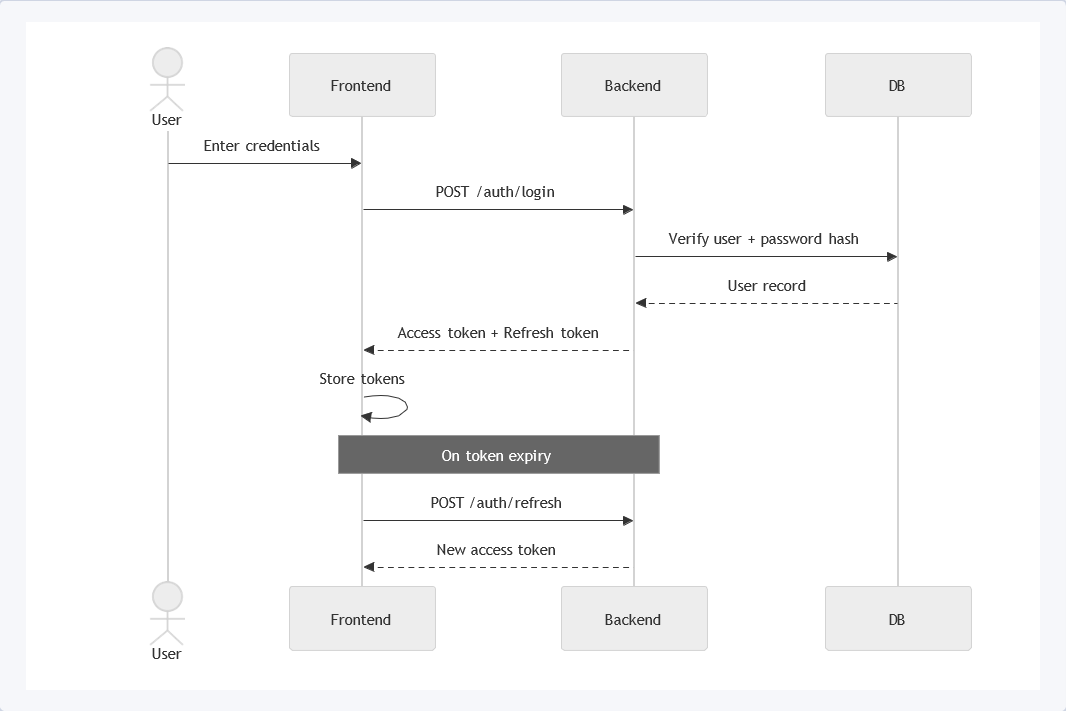
\includegraphics[width=\textwidth]{chapters/chapter05/images/image4.png}
\caption{Sequence Diagram for the JWT-based authentication flow.}
\label{fig:auth_matrix}
\end{figure}

\section{Entity-Relationship Diagram and Database Indexing}
The database structure is shown in Figure~\ref{fig:er_matrix}. It maps the relationships between Users, the extracted Content, and the generated artifacts stored across the Summaries, Quizzes, Presentations, and Flashcards tables. Foreign key constraints enforce referential integrity between these entities.

\subsection{JSONB Indexing Strategy}
One key design decision was how to store the variable-structure outputs from the LLM (such as quiz questions with different numbers of answer options) inside a relational database. Rather than creating deeply normalized tables with many joins, Lectura stores these outputs in PostgreSQL's JSONB column type.

Unlike plain text JSON, JSONB stores data in a parsed binary format that supports indexing. PostgreSQL can apply Generalized Inverted Indexes (GIN) to JSONB columns, which allows efficient lookups on nested keys. For example, querying all quizzes for a specific user that contain a particular question type does not require scanning every row in the table.

For standard columns like \texttt{created\_at} and \texttt{user\_id}, the system uses B-Tree indexes, which provide logarithmic search time:

\begin{equation}
    T_{\text{search}} \approx O(\log_b n)
\end{equation}

Where $b$ is the branching factor and $n$ is the number of rows. B-Tree indexes work well for scalar values but are not designed for nested JSON structures. By combining B-Tree indexes on relational columns with GIN indexes on JSONB columns, the database can handle both structured queries and flexible AI-generated content efficiently.

\begin{figure}[htbp]
\centering
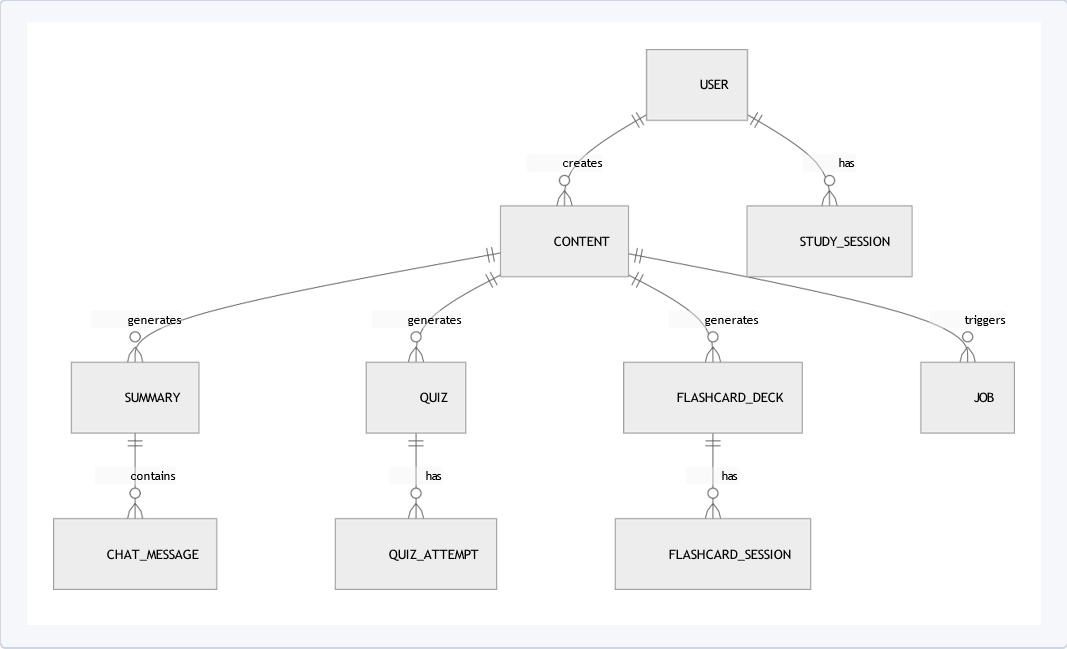
\includegraphics[width=0.9\textwidth]{chapters/chapter05/images/image5.png}
\caption{Entity-Relationship Diagram for the PostgreSQL database schema.}
\label{fig:er_matrix}
\end{figure}

\section{Component Architecture}
At a high level, the system is organized into loosely coupled components. On the frontend, separate modules handle authentication, media upload, and artifact rendering, each managing their own state independently. On the backend, the Go application follows a layered structure: an API router directs requests to handler functions, which call business logic services, which in turn interact with database repositories. The worker pool operates as a separate subsystem that reads from the job queue independently of the main request-handling thread.

\section{Worker Pool Design}
The worker pool is the central mechanism that allows the backend to remain responsive during long-running AI generation tasks. By processing LLM requests in background goroutines rather than in the main HTTP handler, the system achieves several benefits: it can handle many concurrent generation requests without blocking, it isolates slow API responses from affecting other users, it supports automatic retries with exponential backoff when rate limits are hit, and it prevents any single long request from consuming server resources indefinitely. This design is described in more detail in Chapter 4.

\section{Deployment Strategy and CI/CD Pipeline}
To ensure high availability, scalability, and seamless updates, the Lectura platform employs a modern cloud-native deployment strategy. The deployment infrastructure is cleanly separated between the frontend, backend, and database tiers.

\subsection{Frontend Deployment}
The React 18 application is deployed utilizing edge networks such as Vercel. This approach allows the static assets, HTML, CSS, and compiled JavaScript to be distributed globally via a Content Delivery Network (CDN). Continuous integration features provide automatic deployments triggered by Git pushes to the main branch, ensuring that the production environment is always synchronized with the latest validated code.

\subsection{Backend Deployment}
The Go (Golang) backend is containerized using Docker. A \texttt{Dockerfile} defines a multi-stage build process: it first compiles the Go binaries in a comprehensive builder image, and then copies only the compiled executable into a lightweight Alpine Linux container. This reduces the attack surface and minimizes image size. The resulting Docker container is hosted on a cloud Platform-as-a-Service (PaaS). These platforms natively support auto-scaling, horizontal instance replication, and environment variable management for secure injection of the Gemini API keys.

\subsection{Database and Cache Hosting}
The persistent PostgreSQL database and the Redis in-memory cache (used for the worker pool queues and session management) are hosted on managed cloud services. Managed databases were selected over self-hosting to guarantee automated backups, point-in-time recovery, and high availability without introducing significant DevOps administrative overhead.

\subsection{Continuous Integration and Continuous Deployment (CI/CD)}
The CI/CD pipeline is orchestrated via GitHub Actions. Upon every code integration, automated workflows execute unit tests and static code analysis (linting) for both the Go backend and the TypeScript frontend. Once code is merged into the production branch, the CD pipeline automatically triggers the Docker image build, pushes the new image to a container registry, and instructs the production environment to seamlessly roll out the new containers with zero-downtime deployment strategies.